%!TEX root = ../../../adrien_gomar_phd.tex


\begin{figure}[htp]
  \centering
  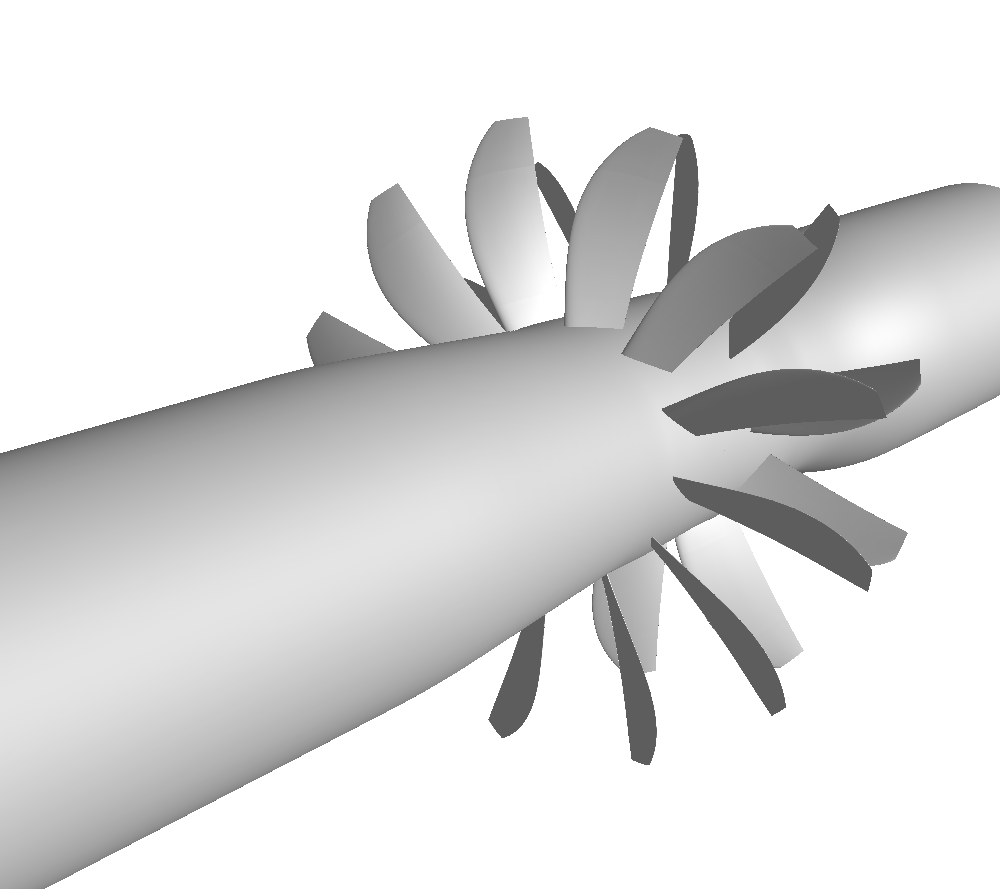
\includegraphics[width=.3\textwidth]{DREAM_LS_wall.png}
  \caption{Low-speed isolated contra-rotating open rotor geometry.}
  \label{fig:dream_ls_wall}
\end{figure}

The studied configuration is a pusher contra-rotating open rotor
that comes from the know-how of Snecma (Safran). 
It is shown in Figure~\ref{fig:dream_ls_wall} for the
Low-speed (LS) flight condition, representative of the take-off
and landing.
The simulated configuration does not include the spinner as the
experimental setup does not take into account this part of the geometry.
The experimental results were not available for comparison
at the time this study was written.

\begin{table}[htp]
  \ra{1.3} \centering
  \begin{tabular}{ccc}
    \toprule
    $M_0$ & $J$ & $M_{tip}$ \\
    \midrule
    $0.2$ & 1.06 & 0.63 \\
    \bottomrule
  \end{tabular}
  \caption{Low-speed isolated contra-rotating open rotor flight condition parameters.}
  \label{tab:dream_ls_flight_condition}
\end{table} 
Table~\ref{tab:dream_ls_flight_condition} recalls the main
parameters of the case: the inflow Mach number $M_0$,
the advance ratio $J$ (see Chap.~\ref{cha:cror})
and the Mach number at the tip of
the front rotor blades $M_{tip}$ based on the inflow 
velocity and the advance ratio
\begin{equation}
  \begin{split}
    M_{tip} &= 
        \sqrt{\frac{V_0^2 + (\Omega R)^2}{\gamma R t_0}} =
        \frac{V_0}{\sqrt{\gamma R t_0}} 
          \sqrt{1 + \left(\frac{\Omega R}{V_0}\right)^2} =
        \frac{V_0}{\sqrt{\gamma R t_0}} 
          \sqrt{1 + \left(\frac{\pi n D}{
          V_0}\right)^2} \\
    &= M_0 \sqrt{1 + \left(\frac{\pi}{J} \right)^2}
  \end{split}
  \label{eq:m_tip}
\end{equation}

At this flight condition, the inflow Mach 
number $M_0$ is within the incompressible range
($M_0 < 0.3$). As the CFD flow solver used here is the
\textit{elsA}~\cite{Cambier2013} CFD code which is a compressible code, 
a preconditionner might be needed for the computations to converge. 
Hopefully, the fluid is accelerated by the two rotors
and the tip Mach number is high enough not to use any preconditionning.
However, let us bare in mind that this range of Mach number might
be tedious for a compressible flow solver.
The advance ratio $J$ is around~1 which is a classical value for
low-speed propellers~\cite{Bousquet2012}. 

Two structural modes are considered for the aeroelastic study of this 
configuration: the second bending/flection mode (2F) 
and the first torsion mode (1T)
of the front rotor. These were inputs of the current work.
The shape of the modes is shown in Figure~\ref{fig:dream_ls_ael_modes}
with an arbitrary amplitude, large enough to ease the visualization.
Two inflection lines are seen for the 2F mode, while only
one is seen for the 1T, hence their designation.
\begin{figure}[htp]
  \centering
  \subfigure[2F]{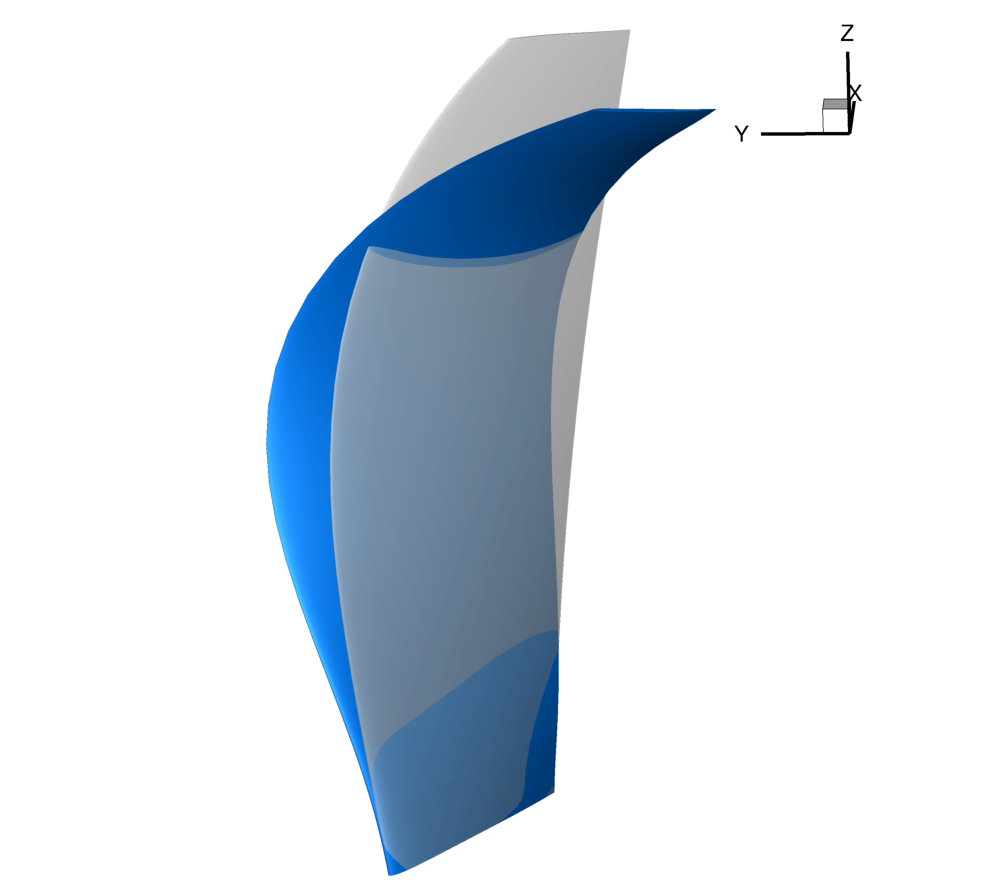
\includegraphics[height=.35\textwidth]{mode_2F.png}}
  \subfigure[1T]{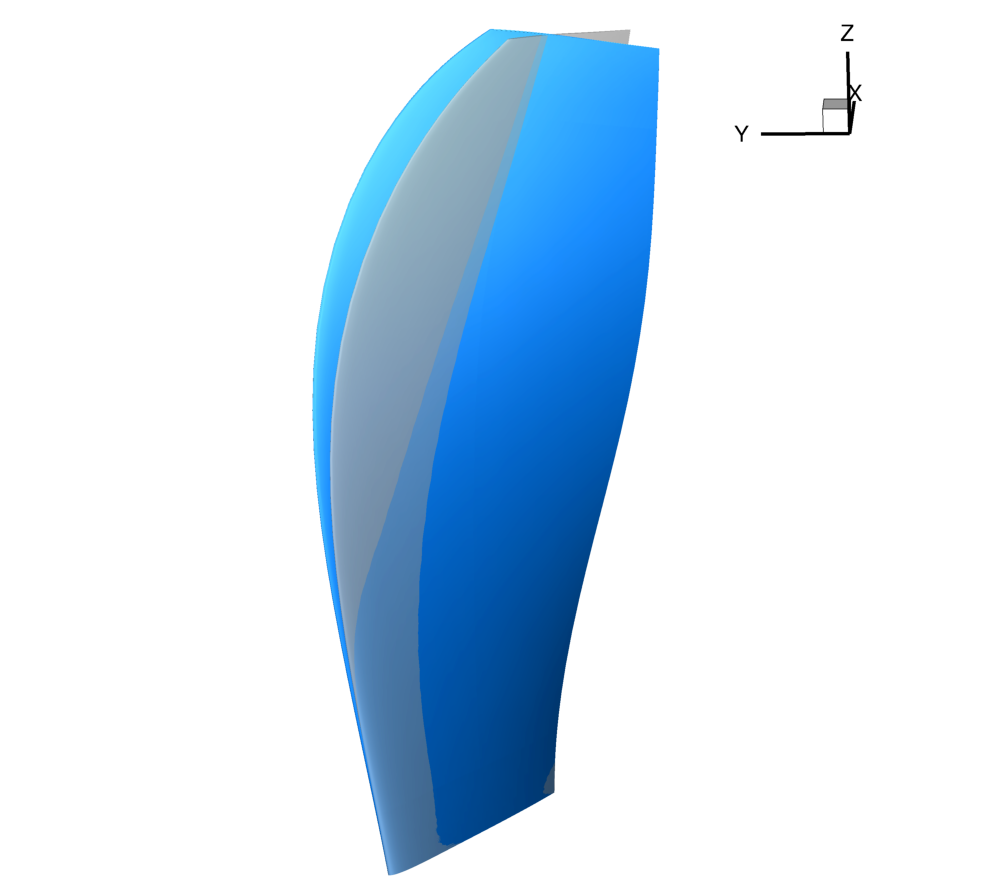
\includegraphics[height=.35\textwidth]{mode_1T.png}}
  \caption{Low-speed isolated configuration: structural modes considered.}
  \label{fig:dream_ls_ael_modes}
\end{figure}
The frequency, mass and stiffness of the modes 
are given with the corresponding modes.
The ratio of the frequency of the blade passing 
frequency of the opposite row, namely the rear rotor,
over the aeroelastic frequency of
each mode varies between 
$3.19 \leq f_{BPF} / f_{AEL} \leq 3.87$. However,
this last frequency governs the unsteady rigid-motion flow physics 
and will have to be computed along with the aeroleastic frequency.
Therefore, the multi-frequential formulation of the
harmonic balance approach will be used to simulate the
aeroelastic response of the blades in Sec.~\ref{sec:dream_ls_ael_results}.
